\section{绘制函数图像}

Lua 计算绘制曲线所需的点，点数由 \tkzname{samples} 选项设置。\TIKZ\ 随后通过这些点连线。

\subsection{定义函数：\tkzcname{tkzFnDef}}

\begin{NewMacroBox}{tkzFnDef}{\marg{名称}\marg{表达式}}
\emph{定义变量为 \texttt{x} 的函数。名称为 Lua 标识符（字母、数字、\texttt{\_}）。之后在所有宏中通过名称引用该函数：\tkzcname{tkzFnDraw}\texttt{(f)}、\tkzcname{tkzFnTangent}\texttt{(f,1)}、\tkzcname{tkzFnArea}\texttt{(f)} 等。在 Lua 中，函数存储在表 \texttt{FN} 中：\texttt{FN.f(2)}。}

\begin{tabular}{lll}
\toprule
参数             & 示例 & 说明  \\
\midrule
\TAline{名称}{f}{函数名}
\TAline{表达式}{x\string^3-2*x}{关于 x 的 Lua 表达式}
\bottomrule
\end{tabular}
\end{NewMacroBox}

\subsection{绘制函数：\tkzcname{tkzFnDraw}}

\begin{NewMacroBox}{tkzFnDraw}{\oarg{选项}\parg{名称} \textrm{或} \oarg{选项}\marg{表达式}}
\emph{函数可以通过名称给出，也可以直接给出表达式；此时用 \tkzname{name} 选项为其命名。}

\begin{tabular}{lll}
\toprule
选项             & 默认值 & 说明     \\
\midrule
\TOline{domain}{xmin:xmax}{绘制区间}
\TOline{samples}{200}{计算点数}
\TOline{name}{}{为函数指定的名称}
\TOline{clip}{true}{曲线裁剪到窗口内}
\TOline{mark=\dots}{}{在每个计算点处放置标记（\tkzname{plotmarks}）}
\TOline{smooth}{}{由 \TIKZ\ 平滑曲线}
\bottomrule
\end{tabular}

\emph{其他选项为 \TIKZ\ 选项；样式为 \tkzname{tkzfn curve}。}
\end{NewMacroBox}

\tkzHand 使用 \tkzcname{tkzFnDraw} 之前，必须先用 \tkzcname{tkzFnInit} 初始化坐标系。

\tkzHand 曲线在函数无定义处中断（如 $x\leq 0$ 时的 |ln(x)|），以及在从窗口一侧跳到另一侧处中断（竖直渐近线）。

%<--------------------------------------------------------------------------->
\subsection{选项：\tkzname{samples}}

画一条线只需两个点：\tkzname{samples=2}。此处请求 400 个点；默认值为 200。

\begin{tkzexample}[latex=7cm]
\begin{tikzpicture}[scale=1]
    \tkzFnInit[xmin=0,xmax=5,
               ymin=0,ymax=2]
    \tkzFnGrid[sub]
    \tkzFnAxes
    \tkzFnDraw[samples=400,
               domain=.5:5]{1/x}
\end{tikzpicture}
\end{tkzexample}

%<--------------------------------------------------------------------------->
\subsection{选项：\tkzname{xstep, ystep}}

\begin{tkzexample}[]
\begin{tikzpicture}
\tkzFnInit[xmin=0,xmax=110,xstep=10,
           ymin=0,ymax=6,ystep=1]
\tkzFnAxisX[label={\textit{年龄}},
            label style={below=12pt,left}]
\tkzFnAxisY[label={\textit{升}}]
\tkzFnDraw[domain=0.1:100]{50/x}
\end{tikzpicture}
\end{tkzexample}

\subsection{调整 \tkzname{xstep} 和 \tkzname{ystep}}

这次定义域从 0 到 700，函数值从 $0$ 到 $\tkzFnPrint{1200}$。使用 \tkzname{tkz-fct} 时，必须用 |\x| 代替 $x$，用 |1./90000| 代替 |1/90000|；现在不再需要。

\begin{tkzexample}[vbox]
\begin{tikzpicture}[scale=1.5]
 \tkzFnInit[xmin=0,xmax=700,xstep=100,
            ymin=0,ymax=1200,ystep=400]
 \tkzFnGrid(0,0)(700,1200)  \tkzFnAxes
 \tkzFnDraw[color=red,samples=100,line width=0.8pt,domain=0:700]
        {(1/90000)*x^3-(1/100)*x^2+(113/36)*x}
\end{tikzpicture}
\end{tkzexample}

\subsection{\tkzname{ystep} 与常函数}

使用 \tkzname{gnuplot} 时，|80/6| 是整数除法，必须写 |80.|；使用 Lua 时，计算始终以小数进行。

\begin{tkzexample}[vbox]
 \begin{tikzpicture}[scale=0.4]
 \tkzFnInit[xmin=0,xmax=30,ymin=0,ymax=90,ystep=6]
 \tkzFnAxisX[ticks=false,label=$t$]
 \tkzFnAxisY[ticks=false,label=$P$]
 \tkzFnDraw[line width=1pt,color=red,dashed,domain=0:30]{80}
 \tkzFnDraw[line width=1pt,color=blue,domain=0:30]{80/(1+4*exp(-0.21*x))}
 \tkzFnText[above,color=red](20,80){$P=80$}
\end{tikzpicture}
\end{tkzexample}

\subsection{一次函数}
画一条线只需两个点：\tkzname{samples=2}。

\begin{tkzexample}[vbox]
 \begin{tikzpicture}[]
 \tkzFnInit[xmin=0,xmax=10,ymin=0,ymax=20,ystep=5]
 \tkzFnAxes
 \tkzFnDraw[color=red,domain=0:10,samples=2]{2*x+5}
 \tkzFnDraw[color=blue,domain=0:10,samples=2]{-x+15}
 \tkzFnDraw[color=green,domain=0:10,samples=2]{7}
\end{tikzpicture}
\end{tkzexample}

%<--------------------------------------------------------------------------->
\subsection{子网格}

   $y=(x-4)\text{e}^{-0.25x+5}$

可以在窗口的一部分区域绘制另一组网格。

\begin{tkzexample}[latex=8cm]
\begin{tikzpicture}[scale=.8]
 \tkzFnInit[xmin=4,xmax=18,xstep=2,
            ymin=20,ymax=90,ystep=10]
 \tkzFnDraw[domain=5:18]
        {(x-4)*exp(-0.25*x+5)}
 \tkzFnGrid(4,20)(18,90)
 \tkzFnAxes
 \tkzFnGrid[sub,
            subdx=0.5,
            subdy=2,
            color=brown](6,60)(12,90)
\end{tikzpicture}
\end{tkzexample}

%<--------------------------------------------------------------------------->
\subsection{文字与点}

\begin{center}
\begin{tkzexample}[vbox]
\begin{tikzpicture}[scale=2]
 \tkzFnInit[xmin=-3,xmax=3,ymin=-1,ymax=4]
 \tkzFnGrid[sub,subdx=.5,subdy=.5]
 \tkzFnAxes
 \tkzFnDraw[domain=-3:2]{(2-x)*exp(x)}
 \tkzFnText(-2,1.25){$\mathcal{C}_{f}$}
 \tkzFnDefPointXY[draw](2,0){A}
 \tkzFnLabelPoints(A)
\end{tikzpicture}
\end{tkzexample}
\end{center}

\endinput
